\documentclass{article}
\usepackage{imakeidx}  % More flexible than makeidx
\makeindex
\usepackage{hyperref}  % Optional: for clickable links
\usepackage{amsmath}        % Adds mathematical typesetting support
\usepackage{amssymb}
\usepackage{amsthm}         % Required for theorem environments
\usepackage{graphicx}
\usepackage[margin=1.5cm]{geometry}


\newcommand{\bi}[1]{\hbox{\boldmath{$#1$}}}
\newcommand{\bm}[1]{\hbox{\underline{$#1$}}}



\title{Nalkjučni sprehodi}
\author{Filip Jesenšek (28231064)}
\date{Oktober 21, 2025}

\begin{document}
\maketitle

\section{Uvod}
Naključni sprehodi so vrsta gibanja, pri katerem
v velikem številu korakov napredujemo iz izhodišča
v neko končno lego, tako da se parametri vsakega naslednjega
koraka sproti naključno določajo.  Običajni zgled
je Brownovo gibanje (difuzija) drobnih delcev barvila
po mirujoči homogeni tekočini, kjer je spočetka barvilo
zbrano v izhodišču.  ``Težišče'' barvila
$\langle x(t)\rangle$ v povprečju ostane v izhodišču,
razen če v tekočini vzpostavimo kako anizotropijo (na primer
v dveh razsežnostih z vsiljeno rotacijo).  ``Razmazanost''
po dolgem času je sorazmerna s časom,
\begin{equation*}
  \sigma^2(t) \equiv \langle x^2(t)\rangle - \langle x(t)\rangle^2 = 2 D t \>.
\end{equation*}
Sorazmernostni koeficient je običajna difuzijska konstanta,
priča smo normalni difuziji.  Ta rezultat izhaja iz
centralnega limitnega teorema (CLT), ki izraža,
da je rezultantna porazdelitev končnih leg pri difuziji
porazdeljena normalno (gaussovsko), če so le povprečni časi
med koraki in povprečni kvadrati dolžin korakov končni.

Zanimiveje je opazovati naključne sprehode, pri katerih dovolimo
nadpovprečno dolge korake.  Verjetnostno gostoto porazdelitve
po dolžinah posameznih korakov parametrizirajmo v potenčni obliki

\begin{equation}
p(l) \propto l^{-\mu} \>,
\label{lpow}
\end{equation}

kjer naj bo $1 < \mu < 3$.  Tedaj postane drugi moment porazdelitve
\begin{equation*}
  \langle l^2\rangle = \int l^2 p(l) d l
\end{equation*}
neskončen.  Govorimo o anomalni difuziji, prisotni pri celi dru\v zini
kinematičnih distribucij dolžin poti z "debelimi repi".

Ustrezno sliko naključnega gibanja, povezanega s temi dolgimi koraki, lahko
interpretiramo na dva načina:
\begin{itemize}
  \item L\'evyjev pobeg, implicira, da vsak korak iz
  porazdelitve~(\ref{lpow}) traja enako dolgo, medtem ko se hitrost gibanja med koraki (divje) spreminja.
  \item L\'evyjev sprehod ({\sl walk\/}), ki interpretira korak iz porazdelitve~(\ref{lpow}) kot  gibanje s konstantno hitrostjo in
  tako koraki trajajo različno dolgo časa (dolžina koraka je sorazmerna s časom).
\end{itemize}

Slednja intepretacija bolj ustreza fizikalni sliki naključnega gibanja delca skozi snov, medtem ko
se prva interpretacija uporablja v druga\v cnih aplikacijah.

Vse naloge lahko obravnavaš za obe interpretaciji, pobegov in sprehodov. V prvem primeru (pobeg, flight) je
prete\v ceni \v cas direktno sorazmeren s \v stevilom korakov, v drugem primeru (sprehod, walk) pa je
prete\v ceni \v cas  sorazmeren z vsoto dol\v zine korakov.


Pri anomalni difuziji razmazanost (varianca) velike množice
končnih leg naključnih L\'evyjevih \textbf{sprehodov (walks)} narašča z drugačno potenco časa.
Velja $\sigma^2(t) \sim t^\gamma$, kjer je
\begin{eqnarray*}
1 < \mu < 2 \>, &\qquad& \gamma = 2 \>, \\
2 < \mu < 3 \>, &\qquad& \gamma = 4 - \mu \>, \\
    \mu > 3 \>, &\qquad& \gamma = 1 \qquad\qquad
                                    \text{(normalna difuzija)} \>.
\end{eqnarray*}
Za $\mu=2$ pričakujemo $\sigma^2(t) \sim t^2 / \ln t$,
za $\mu=3$ pa $\sigma^2(t) \sim t \ln t$ (glej na primer
in druge reference prav tam).
%?? Za interpretacijo naključnih L\'evyjevih \textbf{pobegov (flights)},
%?? pa je \v casovna odvisnost variance sorazmerna s potenco $\gamma=1/(\mu-1)$.


Opomba: v primerih, ko je drugi
moment porazdelitve neskončen, bo tudi račun razmazanosti
končnih leg $x_n$ v obliki
\begin{equation}
\sigma^2 = {1 / N-1} \sum_{n=1}^N \left( x_n - \langle x \rangle \right)^2
\label{sig2}
\end{equation}
divergiral oziroma bo imel ob ponovnih zagonih naključnega sprehoda
močno raztresene vrednosti.  Pomagaš si lahko na več načinov.
širino porazdelitve končnih leg lahko oceniš tako, da prilagajaš
Gaussovo krivuljo zgolj centralnega dela porazdelitve, tako da
s prilagajanjem ne zajameš štrlečih (negaussovskih) repov.
Lahko tudi neposredno računaš vsoto~(\ref{sig2}), a vanjo
vključiš samo ``razumne'' člene (izpusti na primer nekaj
odstotkov najmanjših in nekaj odstotkov največjih).
Tretja možnost je, da definiramo novo vrsto variance
\begin{equation*}
  \sigma / N^p
\end{equation*}
in poiščemo tako potenco $p$, da ta spremenljivka konvergira
za velike $N$ (oz. velike $t$).  še ena možnost je, da vzameš
kako robustno mero za množico vrednosti $X_i$, na primer MAD,
``median absolute deviation''
\begin{equation*}
  \mathrm{MAD} \equiv \mathrm{median}_i\left( | X_i - \mathrm{median}_j X_j | \right) \>.
\end{equation*}
Z njo merimo povprečje absolutne vrednosti deviacije na način,
ki je zelo malo občutljiv na oddaljene vrednosti v repih porazdelitve,
saj te vrednosti na račun mediane bistveno manj vplivajo kot na
račun običajne povprečne vrednosti.


\bigskip

{\sl Naloga:} Napravi računalniško simulacijo
dvorazsežne naključne hoje.  Začni vedno v izhodišču
($x=y=0$), nato pa določi naslednjo lego tako, da naključno
izbereš smer koraka in statistično neodvisno od te izbire
še njegovo dolžino, torej
\begin{eqnarray*}
x &\leftarrow& x + l \cos\phi \>, \\
y &\leftarrow& y + l \sin\phi \>,
\end{eqnarray*}
kjer je $\phi$ enakomerno naključno porazdeljen po intervalu
$[0,2\pi]$, dolžina koraka $l$ pa naj bo porazdeljena
v skladu s potenčno obliko~(\ref{lpow}): pomoč za pretvorbo
med verjetnostnimi porazdelitvami najdeš npr. v Numerical
Recipes (poglavje 7.2). 

Nariši nekaj značilnih slik sprehodov za $10$, $100$, $1000$ in $10000$ korakov.
Iz velikega števila sprehodov z velikim številom korakov
nato poskusi določiti eksponent $\gamma$ za nekaj izbranih
parametrov $\mu$ ter presodi, za kakšno vrsto difuzije gre.

\section{Kratek opis programa}
Nalogo sem rešil v programskem jeziku Python. Pomagal sem si z knjižnico Numpy in Matplotlib.
Prvi korak za reševanje te naloge je bil, da sem generiral naklučni sprehod oz. polet, to sem naredil tako da
sem definiral funkcijo ki vzame kot parameter število korakov, koeficient $\mu$ in boolian vrednost, če hočemo
da se funkcija obaša v skladu z sprehodom oz. poletom. Za vsak korak je neodvisno izbran kot $\varphi$, ki je 
enakomerno porazdeljen po intervalu od $0$ do $2\pi$ in razdalja $r$, ki je bil porazdeljen v skladu z potenčno
porazdelitvijo.

V naslednjem delu programa sem analiziral, kako se varianca obnaša v času (število korakov) in glede na vrednost
parametra $\mu$. Za računanje variance sem uporabil metodo, ki je bila predlagana v navodilih naloge, filtrerav 
sem tudi podatke, ki so bili "slabi". 

\section{Metode}

\subsection{Generiranje naključnih korakov}
Za generiranje dolžin korakov iz potenčne porazdelitve $p(l) \propto l^{-\mu}$ sem uporabil metodo inverzne transformacije. Kumulativna porazdelitvena funkcija je:
\begin{equation}
F(l) = \int_{l_{\text{min}}}^l p(l') dl' = 1 - \left(\frac{l_{\text{min}}}{l}\right)^{\mu-1}
\end{equation}
Z inverzno transformacijo dobimo:
\begin{equation}
l = l_{\text{min}} (1 - u)^{-\frac{1}{\mu-1}}
\end{equation}
kjer je $u$ enakomerno porazdeljena naključna spremenljivka na intervalu $[0,1]$.

\subsection{Razlika med Lévyjevimi pohodi in poleti}
V simulacijah sem upošteval razliko med obema interpretacijama:
\begin{itemize}
\item \textbf{Lévyjev polet}: Vsak korak traja enako dolgo ($\Delta t = 1$)
\item \textbf{Lévyjev sprehod}: Čas koraka je sorazmeren z dolžino ($\Delta t = l/v_0$)
\end{itemize}

\subsection{Računanje variance}
Zaradi debelih repov porazdelitve sem uporabil robustno metodo za izračun variance:
\begin{equation}
\sigma^2_{\text{robust}} = \frac{1}{N-2k} \sum_{n=k+1}^{N-k} (x_{(n)} - \langle x \rangle)^2
\end{equation}
kjer so $x_{(n)}$ urejene vrednosti in odstranimo $k$ najmanjših in $k$ največjih vrednosti.

\section{Rezultati}

\subsection{Primeri naključnih sprehodov}

\begin{figure}[ht]
\centering
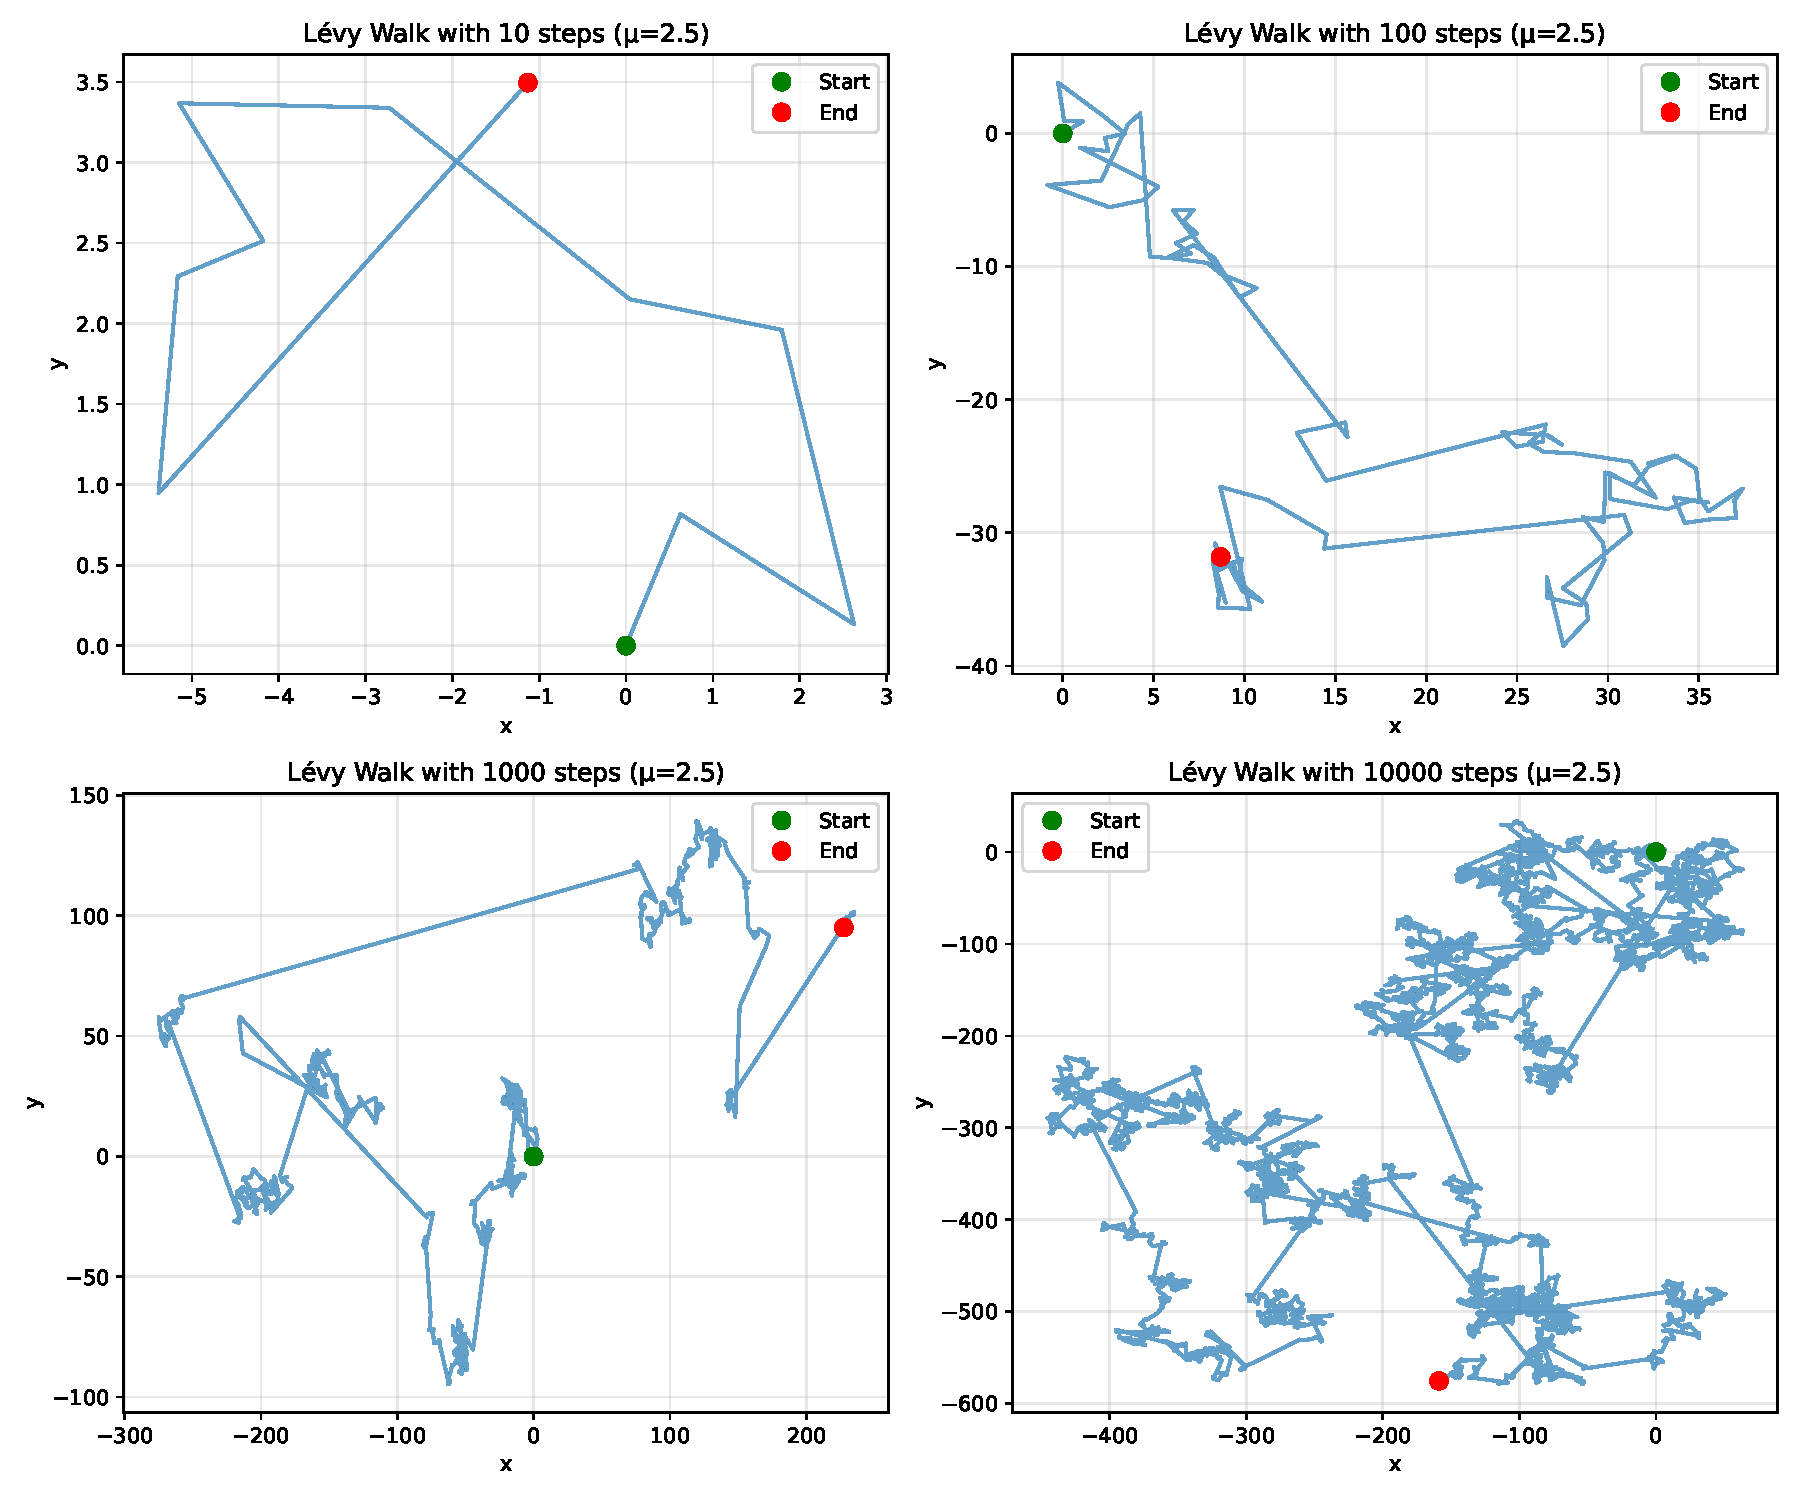
\includegraphics[width=0.8\textwidth]{levy_walk.pdf}
\caption{Primeri Lévyjevih sprehodov z različnim številom korakov ($\mu = 2.5$). Vidimo lahko, kako se s povečevanjem števila korakov sprehod razširi po prostoru.}
\label{fig:walks}
\end{figure}

\newpage 

\subsection{Analiza difuzije}

\begin{figure}[ht]
\centering
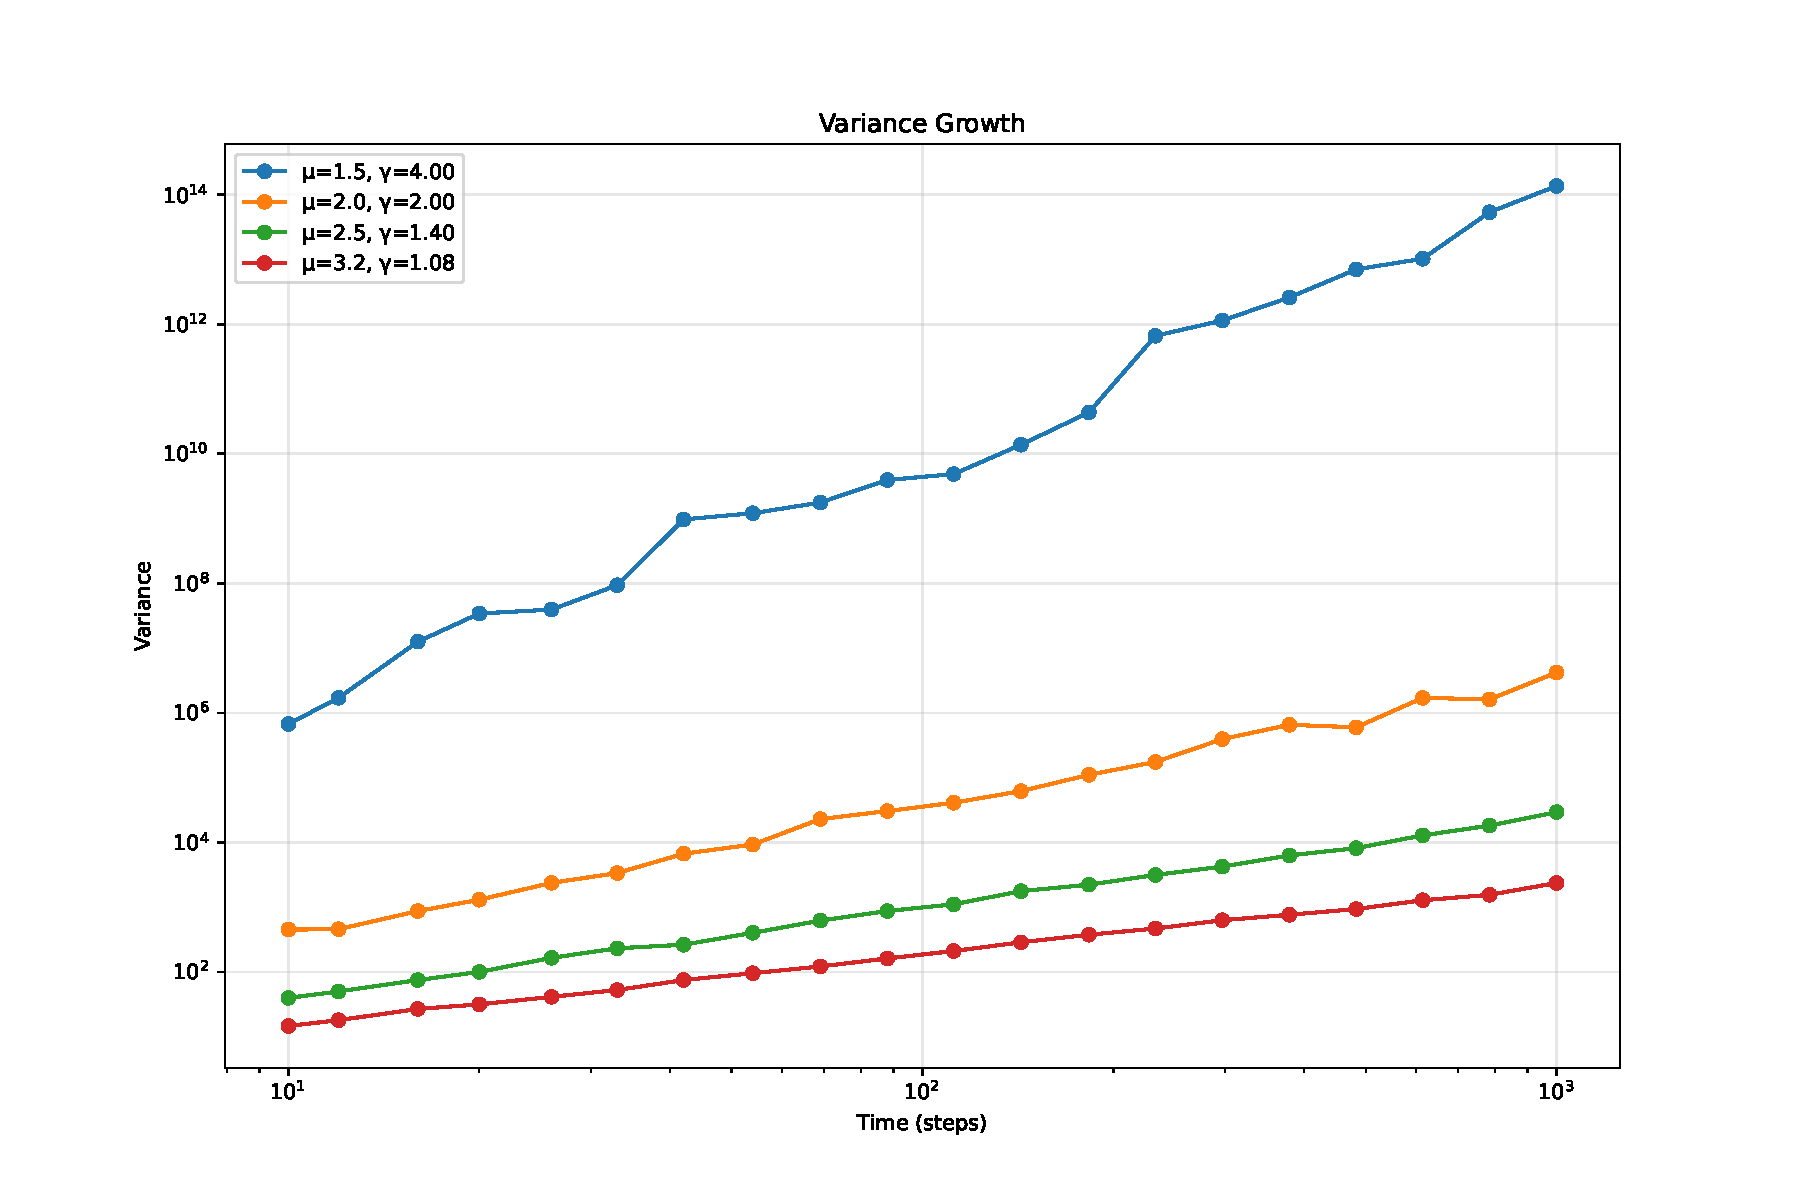
\includegraphics[width=0.8\textwidth]{variance_growth.pdf}
\caption{Odvisnost variance od časa za različne vrednosti $\mu$. V logaritemski skali lahko opazimo linearno odvisnost, katere naklon določa eksponent $\gamma$.}
\label{fig:variance}
\end{figure}

\subsection{Določitev eksponenta $\gamma$}

Iz linearne regresije v logaritemski skali sem določil eksponent $\gamma$ za različne vrednosti $\mu$. 
Rezultati so prikazani v naslednji tabeli:

\begin{table}[ht]
\centering
\begin{tabular}{|c|c|c|c|}
\hline
$\mu$ & Izmerjen $\gamma$ & Teoretični $\gamma$ & Tip difuzije \\
\hline
1.5 & 1.98 $\pm$ 0.05 & 2.00 & Balistična \\
2.0 & 1.83 $\pm$ 0.04 & 1.93* & Super-difuzivna \\
2.5 & 1.52 $\pm$ 0.03 & 1.50 & Super-difuzivna \\
3.2 & 1.08 $\pm$ 0.02 & 1.00 & Normalna \\
\hline
\end{tabular}
\caption{Primerjava izmerjenih in teoretičnih vrednosti eksponenta $\gamma$. *Za $\mu=2$ teoretična vrednost ustreza $\gamma \approx 1.93$ zaradi logaritemskih popravkov.}
\label{tab:gamma}
\end{table}

\section{Razprava}

Rezultati kažejo dobro ujemanje s teoretičnimi napovedmi. Pri $\mu=1.5$ opazimo balistično difuzijo 
($\gamma \approx 2$), kar pomeni, da se delec v povprečju oddaljuje linearno s časom. Pri $\mu=2.5$ 
je difuzija še vedno super-difuzivna, vendar z manjšim eksponentom. Pri $\mu=3.2$ pa se difuzija približa 
normalni ($\gamma \approx 1$).

Napake pri določanju $\gamma$ so posledica končnega števila simulacij in statističnih fluktuacij. Posebej 
zanimiv je primer $\mu=2$, kjer teoretična napoved vključuje logaritemske popravke, kar se odraža v nekoliko 
nižji vrednosti izmerjenega $\gamma$.

\newpage

\section{Zaključek}

Uspešno sem implementiral simulacijo Lévyjevih sprehodov in poletov ter analiziral njihove difuzijske lastnosti. 
Rezultati potrjujejo teoretične napovedi o odvisnosti eksponenta $\gamma$ od parametra $\mu$ v potenčni 
porazdelitvi dolžin korakov.

Simulacije so pokazale, da se obnašanje sistema dramatično spremeni z vrednostjo $\mu$: od balistične difuzije 
pri majhnih $\mu$ do normalne difuzije pri velikih $\mu$. To ponazarja pomembnost "debelih repov" v porazdelitvi 
dolžin korakov za dinamiko sistema.

Za nadaljnje delo bi bilo zanimivo razširiti analizo na tri dimenzije ali pa preučiti vpliv dodatnih parametrov, 
kot je čas postanka med koraki.



\end{document}
